%%%%%%%%%%%%%%%%%%%%%%%%%%%%%%%%%%%%%%%%%
% Short Sectioned Assignment LaTeX Template Version 1.0 (5/5/12)
% This template has been downloaded from: http://www.LaTeXTemplates.com
% Original author:  Frits Wenneker (http://www.howtotex.com)
% License: CC BY-NC-SA 3.0 (http://creativecommons.org/licenses/by-nc-sa/3.0/)
%%%%%%%%%%%%%%%%%%%%%%%%%%%%%%%%%%%%%%%%%

% \documentclass[paper=a4, fontsize=11pt]{scrartcl} % A4 paper and 11pt font size
\documentclass[11pt, a4paper]{book}
\usepackage[T1]{fontenc} % Use 8-bit encoding that has 256 glyphs
\usepackage[utf8]{inputenc}
\usepackage{fourier} % Use the Adobe Utopia font for the document - comment this line to return to the LaTeX default
\usepackage{listings} % para insertar código con formato similar al editor
\usepackage[spanish, es-tabla]{babel} % Selecciona el español para palabras introducidas automáticamente, p.ej. "septiembre" en la fecha y especifica que se use la palabra Tabla en vez de Cuadro
\usepackage{url} % ,href} %para incluir URLs e hipervínculos dentro del texto (aunque hay que instalar href)
\usepackage{graphics,graphicx, float} %para incluir imágenes y colocarlas
\usepackage[gen]{eurosym} %para incluir el símbolo del euro
\usepackage{cite} %para incluir citas del archivo <nombre>.bib
\usepackage{enumerate}
\usepackage{hyperref}
\usepackage{graphicx}
\usepackage{tabularx}
\usepackage{booktabs}

\usepackage[table,xcdraw]{xcolor}
\hypersetup{
	colorlinks=true,	% false: boxed links; true: colored links
	linkcolor=black,	% color of internal links
	urlcolor=cyan		% color of external links
}
\renewcommand{\familydefault}{\sfdefault}
\usepackage{fancyhdr} % Custom headers and footers
\pagestyle{fancyplain} % Makes all pages in the document conform to the custom headers and footers
\fancyhead[L]{} % Empty left header
\fancyhead[C]{} % Empty center header
\fancyhead[R]{Nazaret Román Guerrero} % My name
\fancyfoot[L]{} % Empty left footer
\fancyfoot[C]{} % Empty center footer
\fancyfoot[R]{\thepage} % Page numbering for right footer
%\renewcommand{\headrulewidth}{0pt} % Remove header underlines
\renewcommand{\footrulewidth}{0pt} % Remove footer underlines
\setlength{\headheight}{13.6pt} % Customize the height of the header

\usepackage{titlesec, blindtext, color}
\definecolor{gray75}{gray}{0.75}
\newcommand{\hsp}{\hspace{20pt}}
\titleformat{\chapter}[hang]{\Huge\bfseries}{\thechapter\hsp\textcolor{gray75}{|}\hsp}{0pt}{\Huge\bfseries}
\setcounter{secnumdepth}{4}
\usepackage[Lenny]{fncychap}


\begin{document}

	% Plantilla portada UGR
	\begin{titlepage}
\newlength{\centeroffset}
\setlength{\centeroffset}{-0.5\oddsidemargin}
\addtolength{\centeroffset}{0.5\evensidemargin}
\thispagestyle{empty}

\noindent\hspace*{\centeroffset}\begin{minipage}{\textwidth}

\centering

\includegraphics[width=0.9\textwidth]{logos/logo_ugr.jpg}\\[1.4cm]

\textsc{ \Large TRABAJO FIN DE GRADO\\[0.2cm]}
\textsc{ GRADO EN INGENIERIA INFORMATICA}\\[1cm]

{\Huge\bfseries Android Shield \\}
\noindent\rule[-1ex]{\textwidth}{3pt}\\[3.5ex]
{\large\bfseries Detector de malware para Android }
\end{minipage}

\vspace{2.5cm}
\noindent\hspace*{\centeroffset}
\begin{minipage}{\textwidth}
\centering

\textbf{Autor}\\ {Nazaret Román Guerrero}\\[2.5ex]
\textbf{Director}\\ {José Antonio Gómez Hernández}\\[2cm]

\includegraphics[width=0.3\textwidth]{logos/etsiit_logo.png}\\[0.1cm]
\textsc{Escuela Técnica Superior de Ingenierías Informática y de Telecomunicación}\\
\textsc{---}\\
Granada, Junio de 2021
\end{minipage}
\end{titlepage}


	% Plantilla prefacio UGR
	\thispagestyle{empty}

\begin{center}
{\large\bfseries Android Shield \\ Detector de malware para Android }\\
\end{center}
\begin{center}
Nazaret Román Guerrero\\
\end{center}

%\vspace{0.7cm}

\vspace{0.5cm}
\noindent{\textbf{Palabras clave}: detector, malware, aplicación, permisos, análisis estático, SVM}
\vspace{0.7cm}

\noindent{\textbf{Resumen}\\

Desde que el sistema operativo de Android se lanzó al mercado en el año 2008, su uso ha crecido hasta alcanzar una cuota de mercado que superaba el 70\% en el enero de 2021. Su amplio uso, tanto en dispositivos móviles como en tabletas, relojes, televisores (\textit{SmartTV}) o, incluso automóviles, ha propiciado también el desarrollo de malware o software malicioso para este sistema.

Android contiene aplicaciones (no nativas) y funcionalidades (nativas) en las distintas capas del sistema operativo para mantener el dispositivo seguro. Mantener el dispositivo y las aplicaciones actualizadas y acceder a sitios seguros son medidas básicas de seguridad, como también lo es la gestión de permisos.

Android cuenta con un amplio conjunto de permisos que controlan el acceso a los distintos componentes hardware o software del dispositivo y las acciones que puede realizar cada aplicación. El sistema de permisos es eficaz para evitar ataques y proteger la privacidad del usuario siempre y cuando no se conceda acceso libre a aplicaciones que no deberían solicitar ciertos permisos considerados peligrosos.

En este trabajo nos centramos en analizar los permisos peligrosos solicitados por cada aplicación con la intención de determinar si es una aplicación inofensiva o, por el contrario, se trata de una aplicación maliciosa que se ha colado en nuestro sistema. Haciendo uso del conjunto de permisos que declara cada app, se ha desarrollado una aplicación para Android que detecte los permisos de cada aplicación y, según los permisos peligrosos solicitados, la clasifique en una aplicación benigna o maligna.

Para llevar a cabo esta actividad, se utiliza un modelo de \textit{Machine Learning} que hace uso de los algoritmos PCA y SVM. El PCA selecciona los permisos útiles para la clasificación y el SVM clasifica las aplicaciones según los permisos solicitados, centrándose solamente en aquellos permisos escogidos por el PCA. El modelo entrenado utiliza los permisos extraídos de distintas muestras de aplicaciones, tanto benignas como malignas, para después llevar a cabo la clasificación de nuevas aplicaciones. Con este modelo, el detector \textit{Android Shield} clasifica cada aplicación en benigna o maliciosa, alcanzando un ratio de acierto del 99\%.

\cleardoublepage

\begin{center}
	{\large\bfseries Android Shield: An Android malware detector}\\
\end{center}
\begin{center}
Nazaret Román Guerrero\\
\end{center}
\vspace{0.5cm}
\noindent{\textbf{Keywords}: detector, malware, application, permissions, static analysis, SVM}
\vspace{0.7cm}

\noindent{\textbf{Abstract}\\

Since the Android OS was launched on the market in 2008, its use has grown to reach a market share that exceeded 70\% in January 2021. Its wide use, both on mobile devices and tablets, smartwatches, smart TVs or even cars, has also led to the development of malware or malicious software for this system.

Android contains non-native applications and native functionalities in the different layers of the OS to keep the device safe and sound. Keeping the device and applications up-to-date and accessing only secure sites are basic security measures, as it is managing permissions.

Android has a wide set of permissions that control access to the different hardware or software components of the device and the actions that each application can perform. The permission system is effective in preventing attacks and protecting the user privacy as long as free access is not granted to applications that should not request certain permissions considered dangerous.

In this work we focus on analyzing the dangerous permissions requested by each application with the intention of determining whether it is a harmless application or, on the contrary, it is a malicious application that has crept into our system. Using the set of permissions declared by each app, an Android application has been developed to detect the permissions of each application and, according to the dangerous permissions requested, the app classifies each app into a benign or a malicious one.

To carry out this activity, a \textit{Machine Learning} model is used that makes use of the PCA and SVM algorithms. The PCA selects the useful permissions for classification and the SVM classifies the applications according to the requested permissions, focusing only on those permissions chosen by the PCA. The trained model uses the permissions extracted from different samples of applications, both benign and malware, and then carries out the classification of new applications. With this model, \textit{Android Shield} classifies each application as benign or malicious, reaching a success rate of 99\%.

\cleardoublepage

\chapter*{}
\thispagestyle{empty}

\noindent\rule[-1ex]{\textwidth}{2pt}\\[4.5ex]

D. \textbf{José Antonio Gómez Hernández}, Profesor del Departamento de Lenguajes y Sistemas Informáticos de la Universidad de Granada.

\vspace{0.5cm}

\textbf{Informa:}

\vspace{0.5cm}

Que el presente trabajo, titulado \textit{\textbf{Android Shield, Detector de malware para Android}},
ha sido realizado bajo su supervisión por \textbf{Nazaret Román Guerrero}, y autorizamos la defensa de dicho trabajo ante el tribunal que corresponda.

\vspace{0.5cm}

Y para que conste, expiden y firman el presente informe en Granada a 8 de julio de 2021 .

\vspace{1cm}

\textbf{El director:}

\vspace{5cm}

\noindent \textbf{José Antonio Gómez Hernández}

%\chapter*{Agradecimientos}
%\thispagestyle{empty}
%\vspace{1cm}

	% Índice de contenidos
	%\newpage
	\tableofcontents

	% Índice de imágenes y tablas
	% \newpage
	% \listoffigures

	% Si hay suficientes se incluirá dicho índice
	% \listoftables 
	% \newpage

	% Introducción 
	\chapter{Introducción}

\section{Un poco de historia}

Desde que se lanzó en el año 2008 de la mano de la empresa taiwanesa HTC, el sistema operativo \textbf{Android}, desarrollado por Android Inc. y más tarde adquirido por Google,  ha extendido su uso alrededor de todo el mundo y actualmente cuenta con no menos de 3000 millones de dispositivos que dependen directamente de él, superando con creces su principal competidor iOS, de Apple.

Basado en núcleo de Linux, el código fuente de Android es \textit{Open Source} (conocido como \textit{Android Open Source Project} o \textit{AOSP}) y está licenciado bajo la Licencia Apache.

En 2005, Google compró Android Inc. y dos años más tarde, en 2007, se creó la \textit{Open Handset Alliance}, un conjunto de fabricantes y desarrolladores de hardware, software y operadores de servicio que, junto a Google, lanzaron al mercado la primera versión del sistema operativo (Android 1.0: Apple Pie). No obstante, no fue hasta 2008 cuando apareció el primer teléfono inteligente, el HTC Dream, que utilizaba este sistema operativo.

Desde ese momento, el sistema operativo fue creciendo y desarrollándose cada vez más hasta alcanzar la versión actual, Android 11.

\section{Uso del sistema operativo Android}

Los dispositivos tecnológicos portables, en concreto los teléfonos inteligentes, se han convertido en un pilar fundamental de nuestra vida. A través de estos dispositivos somos capaces de buscar información, mantener el contacto con gente de alrededor de todo el mundo a través de llamadas de teléfono o mensajería instantánea e incluso hacer compras por Internet. Esto ha supuesto un gran avance en materia de comunicaciones y desarrollo de software, pero también ha potenciado el desarrollo de software malicioso, maligno o malware que pone en peligro la seguridad de nuestros datos personales como la localización, los datos bancarios o la información de contacto. 

Android es un sistema con una arquitectura por capas que aisla unas partes del dispositivo de otras y facilita la abstracción en cuanto a programación de aplicaciones. Esto dificulta los ataques en gran medida, pero a pesar de ser robusto, el sistema operativo puede contener agujeros de seguridad que los atacantes pueden utilizar. Su frecuencia de actualización recomendada es mensual, publicandose parches de seguridad de manera continuada para cubrir las vulnerabilidades encontradas y mantener el dispositivo, y por tanto, los datos, a salvo.

A pesar de ello, los atacantes aprovechan los puntos débiles y las vulnerabilidades del día cero (\textit{zero-day vulnerabilities}) para acceder a los dispositivos de una forma u otra y extraer información, por lo general con objetivos económicos.

Entre las medidas de seguridad con las que cuenta Android, destaca su amplio conjunto de permisos. El acceso a las distintas partes del dispositivo, las acciones que se pueden realizar sobre los datos o la recogida y eliminación de información están estrictamente controladas por este sistema. Dentro del conjunto de permisos hay algunos considerados \underline{peligrosos} o \underline{arriesgados} (\textit{risky permissions}). Mediante el control riguroso de estos permisos, el sistema de seguridad de Android se ve reforzado y es eficaz para detener posibles amenazas... siempre y cuando el usuario sea consciente de los permisos que da a las distintas aplicaciones.

Es aquí donde los atacantes pueden sacar provecho de las vulnerabilidades del sistema. Si un usuario descarga una aplicación de una fuente no segura y concede ciertos permisos sin detenerse a pensar qué uso hará la aplicación con la información contenida en su sistema, los atacantes podrán acceder a todas aquellas partes del dispositivo que deseen, extraer toda la información que quieran, hacer llamadas de teléfono, enviar mensajes SMS o recolectar información sobre los contactos del usuario.

\section{Objetivo de este proyecto}

La idea principal de este proyecto es crear una aplicación que ayude a mejorar la seguridad del dispositivo Android haciendo una clasificación de las demás aplicaciones instaladas en aplicaciones benignas o malware. Para ello, utilizando los permisos declarados en el \textsc{Manifest.xml}, se ha entrenado un modelo que clasifique dichas aplicaciones y muestre la estimación hecha para que el usuario sepa si su sistema es vulnerable a amenazas causadas por malware camuflado en forma de aplicación.

poniendo de manifiesto qué 

	% Descripción del problema y hasta donde se llega
	\chapter{Descripción del problema}

Como bien sabemos, los teléfonos móviles son un punto de acceso a gran cantidad de nuestros datos personales, y, al igual que cualquier otro dispositivo, son vulnerables a los ataques cibernéticos que comprometen la privacidad y seguridad de dichos datos. Es inevitable que los dispositivos presenten alguna vulnerabilidad que los atacantes puedan usar, por pequeña que sea. No obstante, en la medida de lo posible, es conveniente mantener el dispositivo actualizado y controlado para minimizar los riesgos presentes y dificultar la entrada a atacantes a nuestro sistema. También es importante instalar aplicaciones de fuentes seguras que no supongan un peligro añadido.

Muchas veces las aplicaciones maliciosas se camuflan entre las aplicaciones benignas y pasan los controles de seguridad de \textit{Play Protect}, pues a simple vista parecen inofensivas. Difundir malware es muy sencillo: solo hay que ocultar con funcionalidades falsas la verdadera naturaleza de la aplicación. Eso ha hecho que las aplicaciones malware se extiendan casi sin control, en muchos casos, sin que los usuarios sean conscientes de que su dispositivo está infectado.

Hay distintos tipos de malware según el tipo de acción que llevan a cabo:

\begin{itemize}
	\item \textbf{Gusanos}: están programados para reproducirse por sí mismos y difundirse a todos los dispositivos que sea posible. Normalmente se transmiten a través de SMS o MMS y no necesitan interacción del usuario para que se ejecuten.
	\item \textbf{Troyanos}: necesitan interacción del usuario en el dispositivo para poder ejecutarse. Se muestran como aplicaciones inofensivas, pero en realidad son programas engañosos que se instalan en nuestro sistema con una misión muy diferente a la que nosotros creemos.
	\item \textbf{Spyware}: recogen la información personal contenida en el dispositivo y la envían a servidores remotos sin el conocimiento ni consentimiento del usuario.
	\item \textbf{Ransomware}: son programas que cifran el dispositivo o los datos contenidos en él para solicitar después un rescate (del inglés, \textit{ransom}, que significa ``rescate''). El pago requerido alcanza cifras muy altas y se suele solicitar en forma de criptomonedas ya que son imposibles de rastrear.
\end{itemize}

Desde que se lanzó en el año 2008 hasta la actualidad, los ataques a teléfonos con sistema operativo Android han aumentado progresivamente con los años, creándose malware cada vez más sofisticado y complejo que pasa desapercibido al ser difícil de detectar. En el siguiente gráfico se puede ver el aumento de \underline{nuevas variantes} de malware entre los años 2010 y principios de 2019.

\begin{figure}[H]
\centering
	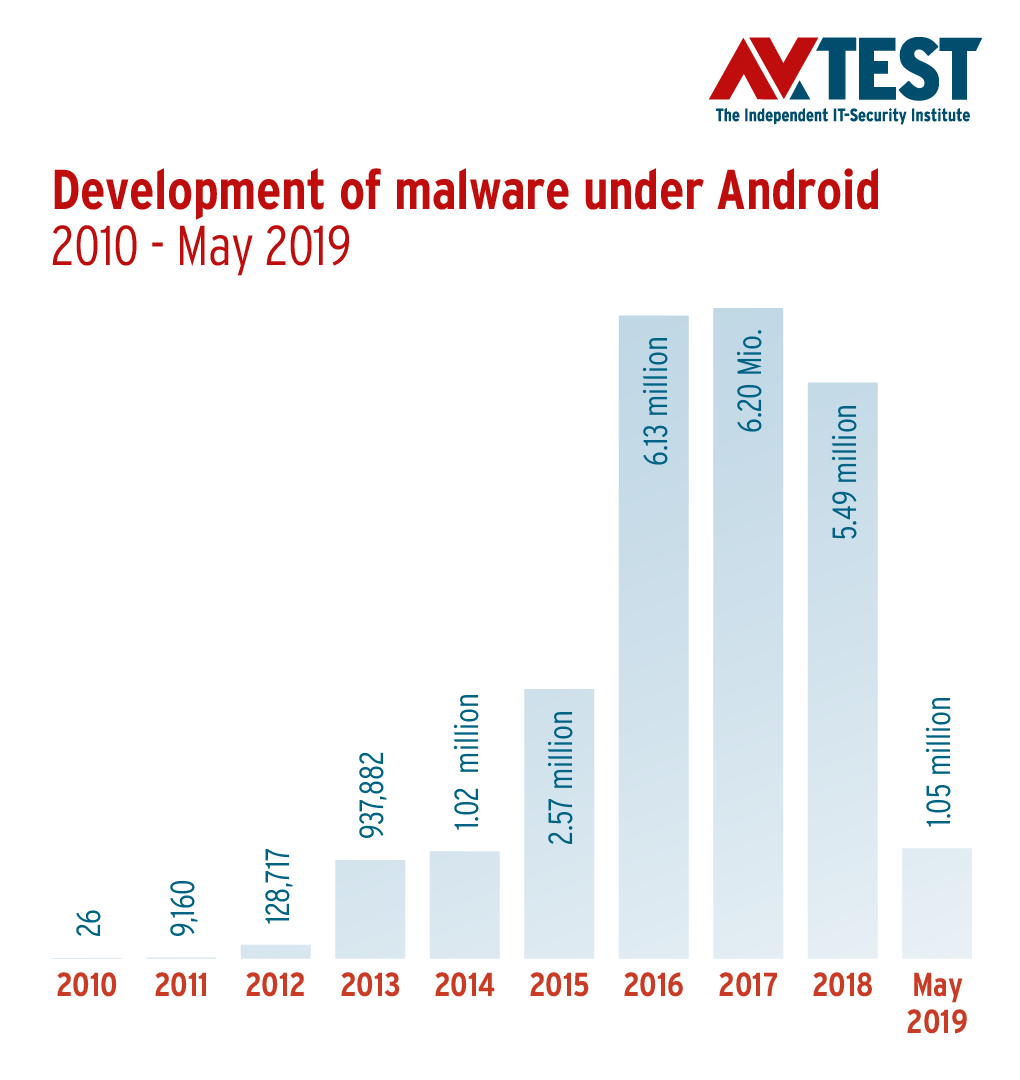
\includegraphics[scale=0.15]{img/2010-mayo2019.png}
	\caption{Nuevo malware desarrollado entre 2010 y mayo de 2019}
\end{figure}

El número de dispositivos infectados durante los dos últimos años supone una cifra preocupante:

\begin{figure}[H]
\centering
	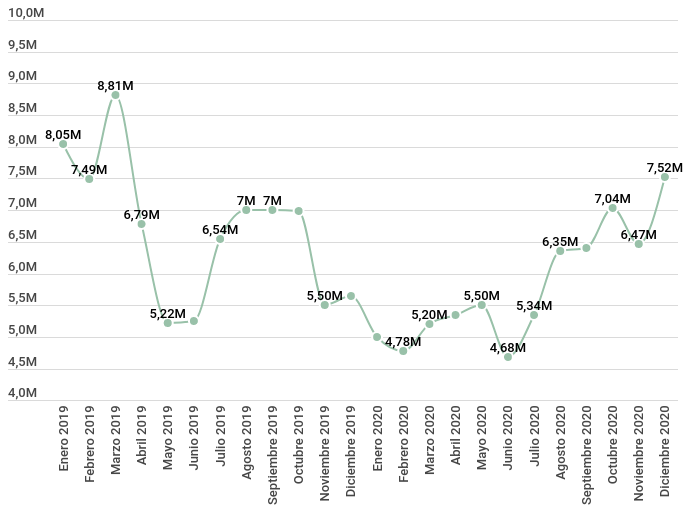
\includegraphics[scale=0.25]{img/2019-2020.png}
	\caption{2019-2020}
\end{figure}

Un indicativo de que la aplicación instalada es un malware (de cualquier tipo) es la cantidad o los tipos de permisos que requiere para su correcto funcionamiento. Las aplicaciones benignas declaran solo los permisos que de verdad necesitan, mientras que un malware declarará más permisos de los que debe y además, por lo general, serán permisos considerados peligrosos. Por ejemplo, en el caso de descargar una aplicación cuya ``funcionalidad'' es la de un bloc de notas, pero que requiere permisos para leer o envíar mensajes SMS, es altamente probable que se trate de un troyano que, o bien recoja datos y los envíe, o bien envíe mensajes que supongan un coste para el usuario.

Hay distintos tipos de análisis para detectar malware según la técnica utilizada:

\begin{itemize}
	\item \textbf{Análisis estático}: es técnica busca malware en la aplicación sin necesidad de ejecutarla. Puede utilizar técnicas de ingeniería inversa para reconstruir el código fuente y buscar comportamientos sospechosos o centrarse en los metadatos de la aplicación e intentar encontrar patrones que puedan indicar que la aplicación es maligna. Hay formas de evitar que el malware sea descubierto mediante este tipo de análisis, como por ejemplo utilizar código ofuscado (que dificulta su lectura comprimiendo y cifrando el malware, añadiendo código muerto, sustituyendo instrucciones por otras equivalentes, etc). La recolección de los permisos de una aplicación para averiguar su clasificación entra en este tipo de análisis.
	\item \textbf{Análisis dinámico}: supone la ejecución del malware en un entorno aislado y controlado (denominado \textit{sandbox environment}) que evitar que el sistema anfitrión en el que se está analizando acabe infectado. Se pueden utilizar depuradores de código para ver la ejecución paso a paso y comprobar los efectos del malware en el sistema. Al igual que en el caso del análisis estático, hay métodos para evitar que la aplicación maligna sea descubierta: detectar si se está ejecutando en un entorno virtual o si el depurador está activo, dificultar, confundir o impedir los volcados de memoria...
\end{itemize}





















	% Estado del arte
	% 	1. Crítica al estado del arte
	% 	2. Propuesta
	\chapter{Estado del arte}

El software libre y sus licencias \cite{gplv3} ha permitido llevar a cabo una expansión del
aprendizaje de la informática sin precedentes.

	
	\chapter{Planificación}

\section{Metodología utilizada}


\section{Temporización}

\section{Seguimiento del desarrollo}


	% Análisis del problema
	% 1. Análisis de requisitos
	% 2. Análisis de las soluciones
	% 3. Solucion propuesta
	% 4. Análisis de seguridad
	\chapter{Análisis del problema}

\section{Solución propuesta}

Como se ha explicado en el Capítulo 1, los peligros del malware en Android son extensos y hay que tener especial cuidado si no queremos que nuestros datos se filtren, sean bloqueados o incluso borrados.

Hemos visto algunos ejemplos de distintas soluciones para detectar malware. Este trabajo se va a centrar en explorar una de ellas, concretamente en una solución que propone un análisis estático que estudia los metadatos de la aplicación contenidos en el \textit{AndroidManifest.xml}: nos vamos a centrar en los permisos peligrosos, aquellos que más arriesgan los datos del usuario. Utilizando la frecuencia con la que las aplicaciones begnigas y el malware utilizan cada uno de estos permisos, se creará un detector en forma de aplicación que clasifique cada aplicación restante instalada en el dispositivo (excepto ella misma) en aplicación benigna o aplicación maliciosa.

En el siguiente capítulo se describirá en detalle la implementación tanto de la aplicación como de los algoritmos utilizados.
 
\section{Análisis de requisitos}

Los requisitos de la aplicación son los siguientes:

\begin{itemize}
	\item \textbf{RF1.} La aplicación debe mostrar el resultado del análisis de las aplicaciones instaladas en el dispositivo.
	\item \textbf{RF2.} Se debe mostrar el nombre de cada app y su correspondiente clasificación.
	\item \textbf{RF3.} El análisis se llevará a cabo solo si el usuario lo solicita.
\end{itemize}

\subsection{Explicación de cada requisito funcional}

\begin{itemize}
	\item \textbf{RF1.} Se mostrará en pantalla un listado de todas las aplicaciones instaladas con su clasificación.
	\item \textbf{RF2.} Para poder identificar cada aplicación se indicará el nombre de ésta además de la etiqueta ``benigna'' o ``maliciosa''.
	\item \textbf{RF3.} El usuario deberá pulsar un botón para activar el análisis. La aplicación nunca funcionará en segundo plano.
\end{itemize}

La estructura a grandes rasgos de la aplicación se puede ver en el siguiente diagrama de clases.

\begin{figure}[H]
\centering
	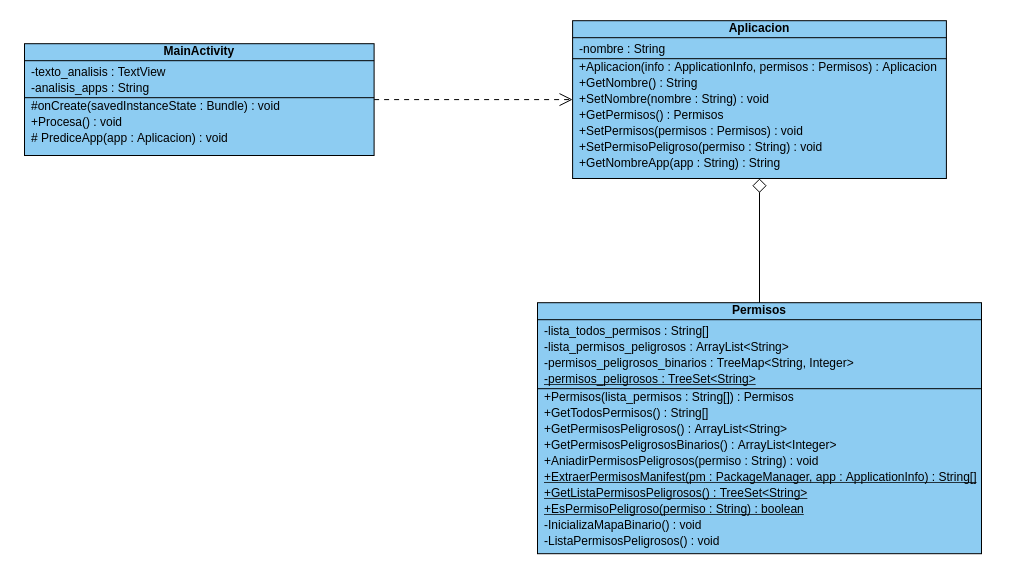
\includegraphics[scale=0.37]{img/uml.png}
	\caption{Diagrama de clases}
\end{figure}

\section{Funcionamiento de los algoritmos de ML}
\label{sec53}

\subsection{Aprendizaje no supervisado: PCA}

El \textit{\href{https://en.wikipedia.org/wiki/Principal_component_analysis}{\textcolor{blue}{Principal Component Analysis}}} o Análisis de Componentes Principales (también llamado PCA), es una técnica que se usa para describir un conjunto de datos en forma de nuevas variables (componentes) que no están relacionadas entre sí. Cada variable da una cantidad de información determinada sobre el problema, por lo que este algoritmo se utiliza para reducir la dimensionalidad del conjunto de datos original; se queda solo con aquellas variables que contienen información suficiente para la resolución del problema.

En este trabajo se ha utilizado la biblioteca \href{https://scikit-learn.org/stable/}{\textcolor{blue}{Scikit Learn}}, que implementa el algoritmo PCA y el SVM. Scikit Learn es una de las bibliotecas de \textit{Machine Learning} más potentes y con mayor variedad de algoritmos disponibles, recomendada para crear modelos ligeros y eficientes que no requieren gran capacidad computacional\hypersetup{citecolor=red}\cite{oreilly}.

Los componentes principales de los datos (representados como un conjunto de puntos en un espacio de coordenadas) son una serie de vectores unitarios donde el vector i-ésimo tiene la dirección de la recta que mejor se ajusta a los datos al mismo tiempo que es ortogonal a los i-1 vectores anteriores. La recta que mejor se ajusta es aquella que minimiza la media de las distancias al cuadrado de los puntos a dicha recta. Esto se traduce en que el PCA cambia ligeramente el conjunto de datos original para quedarse solo con los datos que mejor se ajustan a la recta, lo que significa que en algunas ocasiones se queda solo con unos pocos componentes principales e ignora los demás, manteniendo siempre la mayor variación entre los datos.

En nuestro caso, en este trabajo se ha aplicado el PCA para que el conjunto de permisos original (30 permisos peligrosos) sea reducido de forma que se quede solamente con aquellos permisos que realmente son útiles para diferenciar las aplicaciones entre benignas o maliciosas. Al reducir el número de características, reducimos el ruido que puede confundir al modelo y provocar un sobreajuste a los datos de entrenamiento. Utilizando el PCA nos aseguramos de que el modelo es más genérico.

\subsection{Aprendizaje supervisado: SVM}

Para entrenar el modelo que lleva a cabo la clasificación de las aplicaciones se ha utilizado el algoritmo \textit{\href{https://en.wikipedia.org/wiki/Support-vector_machine}{\textcolor{blue}{Support Vector Machine}}} o Máquina de Vector Soporte, abreviado como SVM. Como se ha explicado ya, este algoritmo es uno de los que mejores resultados arroja en la clasificación de malware. Al igual que para el PCA, se ha utilizado Scikit Learn, por los motivos anteriormente descritos.

El SVM clasifica en dos categorías diferentes un objeto proveniente de un conjunto de datos (de los cuales desconocemos su categoría). Para ello, mediante la búsqueda de un hiperplano separa los datos entre dos subconjuntos con la condición de que debe cumplir con la mayor distancia entre sus fronteras; es decir, se calcula el plano con el cual las distancias de los objetos que hay en el límite de los subconjuntos son máximas. Así, los dos subconjuntos de datos clasificados quedan separados por el hiperplano, uno a cada lado de éste. Se puede ver una representación gráfica en la Figura~\ref{fig:svm}.

\begin{figure}[]
\centering
	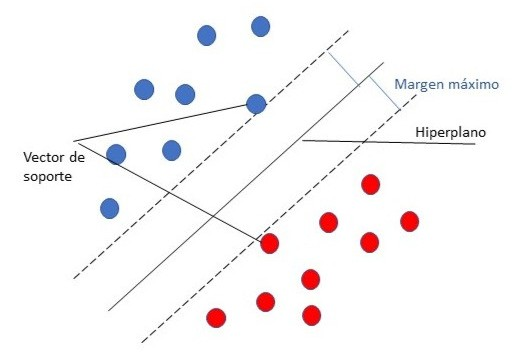
\includegraphics[scale=0.45]{img/svm.jpg}
	\caption{Representación gráfica del funcionamiento del SVM \textit{(Martínez, 2019)}}
	\label{fig:svm}
\end{figure}

Al vector con los los objetos más cercanos al hiperplano se le denomina vector soporte. Las máquinas de vector soporte pueden utilizarse tanto para problemas de regresión como para problemas de clasificación, siendo conceptualmente más apropiados para estos últimos. Están directamente relacionadas con redes neuronales, lo que supone que un modelo bien entrenado suele alcanzar tasas de acierto excelentes. Optimizan la clasificación en dos subconjuntos para crear la mayor diferenciación posible entre categorías. Puesto que este proyecto pretende clasificar una aplicación para hacer que encaje en una de las dos categorías posibles de aplicación (a saber, benigna o maliciosa), este algoritmo es el más adecuado.

Normalmente, no nos encontramos con casos idílicos en los que tenemos dos dimensiones y el hiperplano es recto. Es más, el hiperplano buscado tiene la misma dimensionalidad que el espacio, el cual no tiene por qué ser bidimensional; el número de dimensiones depende del problema concreto (puede llegar a tener infinitas). Además, dependiendo de la distribución de los objetos en el espacio, el hiperplano no tiene por qué ser una línea recta. Puede ser un plano curvo siempre y cuando cumpla con los requisitos de mayor margen entre los objetos frontera y él mismo.

Por tanto, el SVM se enfrenta a varios problemas:

\begin{itemize}
	\item Que haya más de dos variables predictoras en el problema (como es el caso de este trabajo).
	\item Que el hiperplano de separación sea una curva no lineal.
	\item Que los conjuntos no puedan ser totalmente separados ya que, en el caso de serlo, el modelo no puede generalizarse para otros datos (sobreajuste).
	\item Que un objeto pueda ser clasificado en ambas categorías.
\end{itemize}

Por este motivo, el SVM utiliza una \textit{función Kernel} (en este trabajo es una función lineal), que permite convertir un problema de clasificación no lineal en el espacio dimensional original en un problema de clasificación lineal en un espacio dimensional mayor.



	% Desarrollo bajo sprints: 
	% 	1. Permitir registros y login de usuarios
	% 	2. Desarrollo del sistema de incidencias
	% 	3. Desarrollo del sistema de denuncias administrativas y accidentes
	% 	4. Desarrollo del sistema de croquis
	%   5. Instalación de la aplicación de manera automática
	\chapter{Implementación}
\label{cap6}

El desarrollo de la aplicación se ha dividido en diferentes etapas que se explicarán a continuación, según el lenguaje y la funcionalidad que se estaba implementando en cada momento. Todo el código está disponible en \href{https://github.com/nazaretrogue/Android-Shield}{\textcolor{blue}{github.com/nazaretrogue/Android-Shield}}.

\section{Implementación de la aplicación en Java}

La aplicación en sí se implementó en Java por varias razones:

\begin{itemize}
	\item Es el lenguaje oficial de Android. Aunque hay muchas aplicaciones hechas en Kotlin, no está oficialmente respaldado por Google.
	\item Java es un lenguaje orientado a objetos.
	\item Tiene muchas bibliotecas, frameworks y una extensa documentación, lo que facilita la programación y abstrae al programador al llevar a cabo casi cualquier tarea.
	\item El tiempo de ejecución de una aplicación en Java es menor que una aplicación en Kotlin. Además, el tamaño de la biblioteca estándar de Kotlin es mayor, lo que hará que la aplicación pese más que si se hace en Java.
\end{itemize}

La creación de la tarea principal de la aplicación se llevó a cabo en diferentes etapas, empezando por la implementación de la interfaz de usuario. La apariencia de la aplicación es sencilla: una pantalla negra en forma de consola que contiene un cuadro desplazable de texto en el que se escribe en blanco el resultado del análisis. Para activar el análisis de las aplicaciones instaladas hay un botón flotante que inicia el modelo de Python para predecir la clasificación de cada una.

Una vez que la interfaz de usuario estaba construida, se procedió a implementar la actividad en sí. Para ello, se necesitaba un listado de las aplicaciones del dispositivo, así que se utilizó el contexto. El contexto de una aplicación en Android contiene información sobre el entorno en el que la actividad de la app se está desarrollando. A través de él se puede acceder a información del dispositivo como, por ejemplo, el estado actual de la aplicacion en sí, las actividades que se están llevando a cabo en segundo plano o la lista de aplicaciones instaladas en el dispositivo, ente otros.

Se crearon dos clases para modularizar la aplicación:

\begin{enumerate}
	\item \textbf{Clase \textit{Permisos}}: contiene un array con los permisos peligrosos en forma de cadena de cada aplicación y un map con dichos permisos en binario. Hay diferentes métodos para trabajar fácilmente con esta información y abstraerla de la actividad principal.
	\item \textbf{Clase \textit{Aplicacion}}: contiene el nombre y los permisos de cada aplicación. Constituye una unidad sencilla que almacena la información y las operaciones que necesita el detector de malware.
\end{enumerate}

Tras tener las clases implementadas, se procedió a implementar la actividad principal. Ésta utiliza el contexto del detector y extrae todos los permisos de las aplicaciones, que después son filtrados para quedarse solo con los permisos peligrosos. También extrae el nombre de la aplicación para crear un objeto \textit{Aplicacion} que se envía al modelo para que prediga la clasificación.

\section{Implementación de scripts en Python}

A la hora de implementar el modelo a entrenar, las opciones al elegir lenguaje eran mucho más amplias que para hacer la actividad principal, pero se eligió Python por varios motivos:

\begin{itemize}
	\item Es un lenguaje sencillo de entender e implementar.
	\item Hay muchas bibliotecas para desarrollar proyectos de \textit{Machine Learning}, con muchos algoritmos distintos, funcionalidades y herramientas variadas que facilitan la implementación.
	\item Es uno de los  lenguajes con mejor rendimiento a la hora de ejecutar programas que implican \textit{Machine Learning}.
	\item La integración con otros lenguajes es relativamente sencilla.
\end{itemize}

Una vez creada la aplicación, se implementó la parte de Python. A pesar de que no es la actividad principal como tal pues la mayor parte del código no se ejecuta en la app sino antes, esta fase es el grueso de este trabajo.

\subsection{Preprocesador de aplicaciones de muestra}

El primer paso fue implementar un preprocesador para las muestras. El script recibe el \textit{path} en el que están almacenadas las muestras y extrae los permisos de cada aplicación para almacenarlos en un archivo junto con la etiqueta de dicha app.

Se utilizaron un total de 34549 muestras: 14799 aplicaciones malignas y 19750 aplicaciones benignas. Las aplicaciones benignas se extrajeron de la \textit{Play Store}, mientras que las muestras de malware fueron extraídas de distintas bases de datos (Tabla~\ref{tab:dataset}). El archivo con las aplicaciones preprocesadas contiene 31 columnas correspondientes a los 30 permisos peligrosos y a la etiqueta de la aplicación. Los permisos están ordenados por orden alfabético y pueden verse en \textit{\nameref{lista_permisos}}.

\begin{table}[H]
\begin{tabular}{|c|c|c|c|c|}
\hline
\textbf{Nombre} & \textbf{Tipo} & \textbf{Fecha} & \textbf{Nº de muestras} & \textbf{Referencia} \\ \hline
AMD Project     & Malware       & 2018-2019      & 5500                    & \hypersetup{citecolor=red}\cite{amd}                    \\ \hline
Google Play     & Benigna       & 2021           & 19750                   & \hypersetup{citecolor=red}\cite{playstore}                    \\ \hline
VirusShare      & Malware       & 2018-2019      & 8299                    & \hypersetup{citecolor=red}\cite{virusshare}                    \\ \hline
VirusTotal      & Malware       & 2018-2020      & 1000                    & \hypersetup{citecolor=red}\cite{virustotal}                    \\ \hline
\end{tabular}
\caption{Datasets de aplicaciones}
\label{tab:dataset}
\end{table}

\subsection{Script de entrenamiento}

Una vez que las aplicaciones estaban preprocesadas, ya se podía implementar el modelo. Utilizando la biblioteca Scikit Learn, al principio opté por un \textit{Naives Bayes Classifier} (o \textit{Clasificador Bayesiano Ingenuo}), en el que cada característica o \textit{feature} (en este caso cada permiso) es independiente del resto. El algoritmo clasificaba, por tanto, cada aplicación según los permisos que utilizaba sin tener en cuenta la relación entre ellos; por ejemplo, si la mayoría de malware que solicita permiso de lectura de los contactos también solicita permiso de escritura de mensajes SMS, el clasificador ingenuo desecharía dicha relación.

De todas las muestras recogidas, el 80\% de éstas (elegidas aleatoriamente) se utilizó para entrenar al modelo y el 20\% restante se usó para hacer los tests.

Tras entrenar al modelo, la \textit{accuracy} o precisión era de solo un 79\%; para incrementar la precisión, se llevó a cabo un PCA (análisis de componentes principales), una técnica que analiza cada \textit{feature} y elimina aquellas que no son útiles para diferenciar entre aplicación benigna o malware. Es decir, lo que hace la técnica del PCA es eliminar el ruido introducido por las \textit{features} que lo único que hace es ``confundir'' al clasificador. Desgraciadamente, la precisión solo se incrementó hasta alcanzar un 84\%. Para ver mejor el resultado, se generó una curva ROC (Figura~\ref{fig:roc1}), una representación gráfica que muestra la precisión del clasificador.

\begin{figure}[H]
\centering
	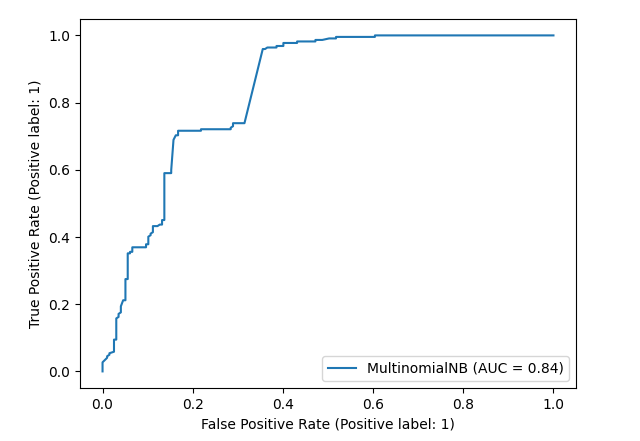
\includegraphics[scale=0.6]{img/roc-84.png}
	\caption{Curva ROC con el clasificador bayesiano}
	\label{fig:roc1}
\end{figure}

Puesto que el resultado no era el esperado, hubo que cambiar de algoritmo. Según el problema al que nos enfrentamos, la selección del algoritmo es fundamental si queremos obtener resultados prometedores\hypersetup{citecolor=red}\cite{oreilly}. Debido a la naturaleza de los datos del problema, el número de \textit{features} (permisos) y el propósito del análisis (la clasificación de aplicaciones), se decidió utilizar un algoritmo algo más complejo y sofisticado como la \textit{Support Vector Machine} o SVM (\textit{Máquina de Vector Soporte}), más apropiado para tratar con el problema de diferenciar entre aplicaciones benignas o malware. Aunque el clasificador bayesiano puede ser efectivo en otros problemas de clasificación, en este en concreto no lo es, pues ignora la relación que puede haber entre dos \textit{features}, lo que se traduce en un decremento de la precisión. SVM no ignora la relación entre \textit{features}, así que la precisión obtenida mejora notablemente.

El SVM es un clasificador capaz de distinguir, en un espacio finito de muestras, entre dos subconjuntos, en este caso entre que la aplicación sea benigna o maligna. El SVM busca un hiperplano para separar ambos subconjuntos según las dimensiones del espacio en el que se encuentran las muestras. Por ejemplo, en un espacio 2D, el SVM buscará una recta que separe ambos subconjuntos y que permita la mayor distancia entre ellos.

Después de hacer los tests, el clasificador SVM junto con la técnica del PCA dio una precisión del 99\%. Se utilizó también \textit{cross-validation}, una técnica que permite comprobar el \textit{overfitting} o sobreajuste del modelo a los datos de entrenamiento.

El resultado, por tanto, era satisfactorio.

\begin{figure}[H]
\centering
	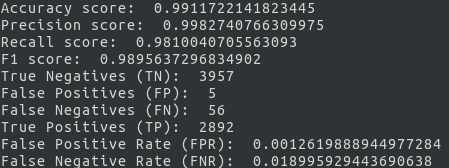
\includegraphics[scale=0.8]{img/accuracy.png}
	\caption{Precisión del modelo entrenado}
\end{figure}

\begin{figure}[H]
\centering
	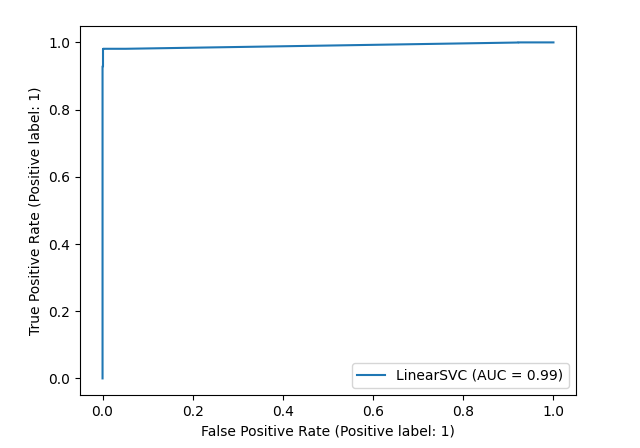
\includegraphics[scale=0.6]{img/roc.png}
	\caption{Curva ROC con el clasificador SVM}
\end{figure}

Una vez obtenidos los resultados deseados, tanto el modelo PCA como el modelo SVM se guardaron en sendos archivos binarios mediante la biblioteca \textit{Pickle} para después poder utilizarlos en el script de predicción.

En la Tabla~\ref{tab:metricas} podemos ver los resultados obtenidos por \textit{Android Shield}:

\begin{itemize}
	\item FPR (\textit{False Positive Rate}) es el porcentaje de falsos positivos, es decir, el número de aplicaciones clasificadas como malware cuando en realidad son aplicaciones benignas.
	\item FNR (\textit{False Negative Rate}) es el porcentaje de falsos negativos, o sea, el número de aplicaciones erróneamente clasificadas como aplicaciones benignas cuando en realidad son malware.
	\item TN (\textit{True Negative}) es el número de aplicaciones clasificadas correctamente como aplicaciones benignas de un total de 6910 aplicaciones utilizadas en los tests.
	\item FP (\textit{False Positive}) es el número de aplicaciones clasificadas erróneamente como malware cuando son benignas.
	\item FN (\textit{False Negative}) es el número de aplicaciones clasificadas erróneamente como aplicaciones benignas cuando en realidad son malware.
	\item TP (\textit{True Positive}) es el número de aplicaciones correctamente clasificadas como malware.
\end{itemize}

\begin{table}[H]
\centering
\begin{tabular}{|c|c|}
\hline
\textbf{Métrica} & \textbf{Resultado}  \\ \hline
Accuracy & 99.11\% \\ \hline
FPR & 0.12\% \\ \hline
FNR & 1.89\% \\ \hline
TN & 3957 \\ \hline
FP & 5 \\ \hline
FN & 56 \\ \hline
TP & 2892 \\ \hline
\end{tabular}
\caption{Resultados de \textit{Android Shield}}
\label{tab:metricas}
\end{table}

\subsection{Script de predicción}

Una vez que el modelo estaba entrenado, se implementó el script en el que se predecía si una app dada era o no malware. Dicho script recibe un nombre de aplicación y el array binario con los permisos peligrosos de dicha aplicación.

En este script, tras cargar el modelo del PCA y el del SVM, se filtran los permisos con el PCA para obetener las \textit{features} que realmente se utilizan para clasificar la app, y una vez hecho esto, se predice la app utilizando el modelo entrenado y éste devuelve la etiqueta de la clasificación.

Antes de integrarlo con la aplicación de \textit{Android Shield}, se hicieron pruebas para comprobar el funcionamiento (razón por la cual hay una función \textbf{main} en dicho script a pesar de no ser necesaria para su ejecución en la aplicación).

\section{Integración Java-Python}

Tras haber comprobado el correcto funcionamiento de modelo, se llevó a cabo la integración entre la aplicación y el modelo. Al ser dos lenguajes diferentes, se necesitaba un soporte extra, como \textit{Weka}, \textit{Jython} o \textit{ApacheSpark}. No obstante, se optó por una opción más sencilla pero de la que fue necesario solicitar una licencia Chaquopy; de esta forma, la integración entre ambos lenguajes no requiere de bibliotecas externas o extensas modificaciones de código.

Con la licencia activada, solo hubo que modificar ligeramente la actividad principal de la aplicación. Durante la creación de la app se tenía que iniciar Python; una vez hecho esto, se debía crear una instancia de Python desde la cual se llamaría al script de predicción con los parámetros solicitados, es decir, el nombre de la app que se está analizando en cada momento y un array con los permisos peligrosos. 

\section{Pruebas}

Una vez que toda la aplicación estaba ensamblada y en funcionamiento con el modelo correctamente entrenado, se hicieron pruebas de funcionamiento. Al abrir la aplicación aparece una pantalla negra, un botón redondo en la esquina inferior derecha y un mensaje en el que se indica que se debe pulsar dicho botón para inciar el análisis de las aplicaciones instaladas.

Una vez pulsado el botón, hay que esperar un par de segundos para que se complete el análisis y se muestren los resultados en pantalla. Cuantas más aplicaciones haya en el dispositivo, más tiempo tardará el análisis. Se muestra en forma de lista en un cuadro de texto desplazable. Tiene el aspecto de la Figura~\ref{fig:prueba}.

Como se puede observar en la Figura~\ref{fig:prueba}, rodeada con un rectángulo de color verde, hay una aplicación señalada como malware: la aplicación de llamadas. La clasificación de esta app es un falso positivo, como es obvio. No obstante, es inevitable que ocurra, ya que la aplicación de llamadas requiere varios permisos considerados peligrosos: acepta llamadas, puede grabar un mensaje de voz para el contestador, responde y hace llamadas, procesa las llamadas salientes, puede leer y escribir en el log de llamadas, leer y escribir contactos y leer y escribir números de teléfono. Esta prueba demuestra que la aplicación funciona bien por lo general pero que hay aplicaciones que, aunque nosotros sabemos que no son malware, \textit{Android Shield} considera maliciosas.

\begin{figure}[H]
\centering
\begin{minipage}{.5\textwidth}
	\centering
	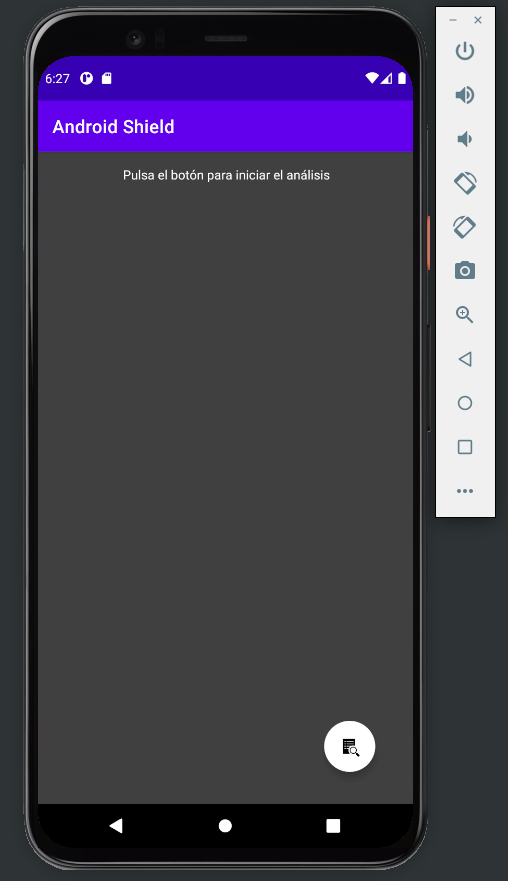
\includegraphics[scale=0.3]{img/emulator.png}
	\captionof{figure}{Pantalla inicial}
	\label{fig:test1}
\end{minipage}%
\begin{minipage}{.5\textwidth}
	\centering
	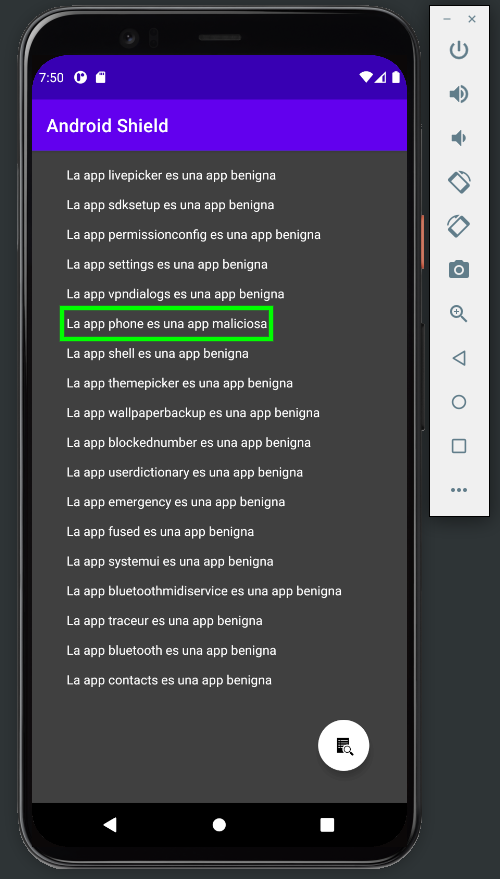
\includegraphics[scale=0.3]{img/test.png}
	\captionof{figure}{Resultado del análisis}
	\label{fig:prueba}
\end{minipage}
\end{figure}

\subsection{Requerimientos del dispositivo}

Ya que el entrenamiento del modelo se lleva a cabo fuera del dispositivo, lo único que hace la actividad principal es cargar dicho modelo para poder analizar las apps instaladas. Eso significa que los costes para ejecutar \textit{Android Shield} son muy bajos y el análisis de malware se lleva a cabo dentro del dispositivo. Esto supone una ventaja frente aquellos detectores de malware que tal vez sean más potentes pero que, debido a los altos requerimientos computacionales, deben llevarse a cabo fuera del dispositivo, como\hypersetup{citecolor=red}\cite{cloud}.

Se han comprobado los requerimientos de CPU, de memoria y de batería de \textit{Android Shield}. La Figura \ref{fig:general} muestra el tiempo de ejecución (alrededor de 4 segundos para analizar 74 aplicaciones, desde el minuto 01:02:00 hasta el 01:06:30 aproximadamente) y el uso de que hace de CPU y memoria durante ese tiempo. También se puede observar que el gasto de batería durante el análisis es mínimo, así que \textit{Android Shield} es una aplicación ligera y que prácticamente no afecta al rendimieto.

\begin{figure}[H]
\centering
	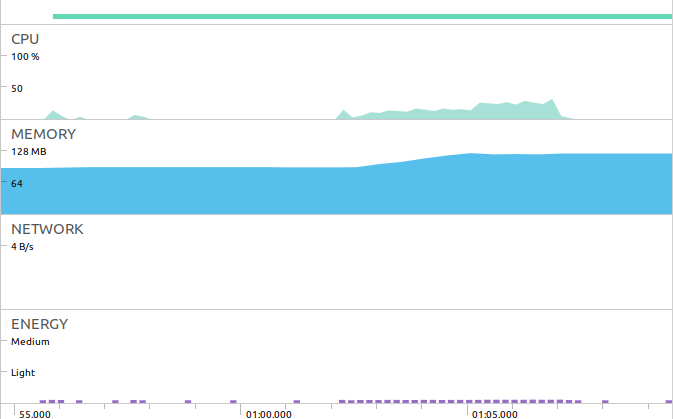
\includegraphics[scale=0.5]{img/general.png}
	\caption{Requerimientos de \textit{Android Shield}}
	\label{fig:general}
\end{figure}

Se ha hecho un zoom en la CPU y en el uso de memoria para que se vea más claramente. En la Figura \ref{fig:memory} además se especifíca para que se está usando la memoria. La mayor parte de la ocupación proviene del propio sistema operativo, aunque cuando se empieza a ejecutar \textit{Android Shield} se muestra un pequeño incremento del uso, que corresponde con la carga del código de Java.

\begin{figure}[H]
\centering
	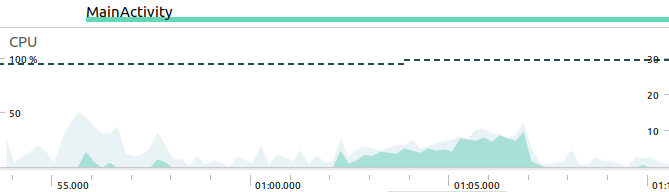
\includegraphics[scale=0.5]{img/cpu.png}
	\caption{Requerimientos de CPU}
	\label{fig:cpu}
\end{figure}

\begin{figure}[H]
\centering
	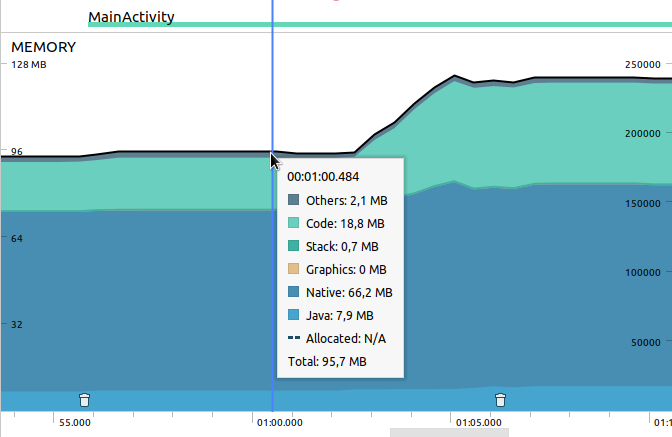
\includegraphics[scale=0.5]{img/memory.png}
	\caption{Requerimientos de memoria}
	\label{fig:memory}
\end{figure}

\section{Mejoras de Android Shield frente a otros trabajos}

Si comparamos este trabajo con otros similares que hemos visto antes, es fácil apreciar que \textit{Android Shield} tiene una precisión superior a todos ellos: 99\% de precisión frente al 85\% de Giang\hypersetup{citecolor=red}\cite{giang}, al 91.8\% de aciertos de Aung\hypersetup{citecolor=red}\cite{aung}, al 93.62\% de precisión de \textit{SIGPID}\hypersetup{citecolor=red}\cite{sigpid} o incluso al que mejores resultados daba, \textit{SFDroid}\hypersetup{citecolor=red}\cite{garg}, con un porcentaje de aciertos del 95.90\%.

Solo Wang\hypersetup{citecolor=red}\cite{cloud} supera la precisión de nuestro trabajo con un 99.71\% de precisión; no obstante, a diferencia de \textit{Android Shield}, Wang lleva a cabo un análisis en la nube, fuera del dispositivo, lo que supone una desventaja.

Por otra parte, \textit{Android Shield} encuentra un punto medio entre el número de permisos utilizados y la precisión alcanzada del modelo. Algunos trabajos utilizan un número muy elevado de permisos para mejorar la precision (como \textit{FDP}\hypersetup{citecolor=red}\cite{jiang}). Analizar un número muy elevado de permisos supone un coste añadido para el dispositivo, que requiere más tiempo de análisis: en este caso tarda alrededor de 15 segundos para analizar 50 aplicaciones.

En el extremo contrario podemos encontrar trabajos que utilizan un conjunto más reducido de permisos. Esto puede ser una ventaja frente a \textit{Android Shield} ya que eliminan ruido que puede confundir al modelo, pero requiere de un preprocesamiento extra, un estudio previo para definir qué permisos son los más útiles para diferenciar entre malware y aplicaciones benignas (como \textit{SIGPID}\hypersetup{citecolor=red}\cite{sigpid}); además, utilizar muy pocos permisos puede afectar a la precisión del modelo como ocurre con Giang\hypersetup{citecolor=red}\cite{giang}.

En cuanto al algoritmo utilizado, hemos comprobado que en \textit{Android Shield} el SVM ha dado unos resultados óptimos, mucho mejores que los demás trabajos. En concreto, \textit{FDP}\hypersetup{citecolor=red}\cite{jiang}, \textit{SIGPID}\hypersetup{citecolor=red}\cite{sigpid} y \hypersetup{citecolor=red}\cite{garg} utilizaban el mismo algoritmo para hacer pruebas, pero, debido a la diferencia de planteamientos, los resultados obtenidos con el algoritmo SVM en estos trabajos no han sido tan buenos como en \textit{Android Shield}. Esto demuestra lo importante que es elegir correctamente las \textit{features} que el modelo va a usar para analizar, pues utilizando el mismo algoritmo los resultados de los tres trabajos mencionados son muy diferentes entre sí, con una clara mejora presentada por \textit{Android Shield}.

Esta comparación se puede ver un poco mejor en la Tabla~\ref{tab:comp-as}.

\begin{table}[H]
\centering
\begin{tabular}{|c|c|c|c|}
\hline
\textbf{Trabajo}        & \textbf{Tipo de análisis}       & \textbf{Algoritmo} & \textbf{Precisión} \\ \hline
\textit{Android Shield} & Estático (on-device)              & PCA + SVM          & 99.11\%               \\ \hline
\hypersetup{citecolor=red}\cite{jiang}                       & Estático (on-device)              & J48                & 94\%               \\ \hline
\hypersetup{citecolor=red}\cite{giang}                       & Estático (on-device)              & Decision tree      & 85\%               \\ \hline
\hypersetup{citecolor=red}\cite{sigpid}                       & Estático (on-device)              & FT                 & 93.62\%            \\ \hline
\hypersetup{citecolor=red}\cite{aung}                       & Estático (on-device)              & K-means clustering & 91.8\%             \\ \hline
\hypersetup{citecolor=red}\cite{cloud}                       & Híbrido (off-device) & SVM + Chi squared  & 99.71\%            \\ \hline
\hypersetup{citecolor=red}\cite{kumar}                       & Estático (on-device) & LSI + Random forest  & 93.92\%            \\ \hline
\hypersetup{citecolor=red}\cite{garg}                       & Estático (on-device) & SVM  & 95.90\%            \\ \hline
\hypersetup{citecolor=red}\cite{todd}                       & Estático (on-device) & Random forest  & 81.53\%            \\ \hline
\end{tabular}
\caption{Comparativa con \textit{Android Shield}}
\label{tab:comp-as}
\end{table}

\section{Tecnologías y bibliotecas utilizadas}

\begin{itemize}
	\item \href{https://developer.android.com/studio}{\textcolor{blue}{AndroidStudio}}: entorno de desarrollo para crear aplicaciones de Android. Cuenta con un emulador de Android (se puede elegir el tipo de dispositivo, la versión de Android...) y una pestaña para que diseñar gráficamente la aplicación sea más cómodo y sencillo.
	\item \href{https://scikit-learn.org/stable/}{\textcolor{blue}{Scikit Learn}}: biblioteca de Machine Learning para Python. Contiene los algoritmos de aprendizaje utilizados (tanto \textit{Naives Bayes} como SVM) así como PCA  y crossvalidation, entre otros.
	\item \href{https://chaquo.com/chaquopy/}{\textcolor{blue}{Chaquopy}}: módulo que permite la integración de Python en aplicaciones Android. Requiere de una licencia, ya sea gratuita para proyectos de código abierto (requiere que el proyecto sea liberado bajo licencia en GitHub o algún otro control de versiones) o de pago para proyectos no libres.
\end{itemize}

	% Presupuesto

	% Conclusiones
	\chapter{Conclusiones y trabajos futuros}

Para terminar, hagamos una pequeña reflexión con todo lo visto, tanto en lo referente a los antecedentes que nos han llevado a desarrollar este trabajo como a trabajo en sí y lo que éste implica.

Los ataques a dispostivos Android son una de las principales amenazas a las que nos enfrentamos a diario. Puesto que nuestros teléfonos móviles son una de las tecnologías más extendidas a lo largo del mundo y una de las más utilizadas cada día, gran parte de nuestra vida está contenida en ellos, lo que nos hace vulnerables y un objetivo atractivo para los atacantes. Nadie está a salvo, aunque creamos que al ser usuarios ``comunes'' no estamos expuestos al mismo peligro que las grandes empresas. Tal vez el riesgo que corremos es menor, pero no es nulo. Es importante mantener el dispositivo actualizado, instalar solo aplicaciones de fuentes confiables y dar y revocar solo los permisos estrictamente necesarios para evitar abrir brechas de seguridad por las que puedan colarse los atacantes.

Como se ha explicado a lo largo de esta memoria, hay diferentes formas de enfocar el problema para evitar lo máximo posible los riesgos a los que nos encontramos expuestos, pero ninguna de estas soluciones es 100\% eficaz. Esto significa que siempre, por muy cuidadosos que seamos, habrá una posibilidad de que nuestro dispositivo sea atacado y nuestros datos, puestos en riesgo. La aproximación que ofrece la aplicación desarrollada en este proyecto es una solución adecuada para la detección de malware en Android sin reducir en exceso el rendimiento del dispositivo, lo que permite que el usuario pueda tomar medidas para eliminar el malware de su teléfono.

A pesar de los errores que pueda cometer en la clasificación, la aplicación de \textit{Android Shield} es una aproximación válida para controlar el dispositivo y saber si ha sido infectado sin que el rendimiento se vea casi afectado. El análisis llevado a cabo muestra una precisión del 99\%, lo que significa que esta aplicación es capaz de detectar la mayor parte del malware mejor que otros trabajos similares, aunque sigue habiendo falsos negativos que pueden ser reducidos para mejorar aún más la precisión.

Una ventaja clara que posee la aplicación es que utiliza un análisis estático, lo que significa que no requiere la engorrosa tarea de ejecutar previamente en un entorno aislado la aplicación sospechosa de ser malware. Además, al llevarse a cabo el análisis dentro del dispositivo, la ejecución es más rápida.

El objetivo principal para mejorar la aplicación es conseguir que detecte malware del día cero. Se podría continuar desarrollando la aplicación para mejorar el análisis con más experimentación y ajustando los parámetros del algoritmo, de manera que también fuera capaz de detectar malware que nunca había aparecido antes y que cuenta con una combinación de permisos declarados que el modelo entrenado no ha visto.

Para mejorar más \textit{Android Shield}, se podría hacer más atractiva la interfaz de usuario y añadir nuevas opciones de análisis, como por ejemplo, en el caso de que un usuario instale una nueva aplicación y quiera analizarla pero ya haya analizado el resto de apps de su dispositivo, se podría añadir una opción en la que se elija qué aplicaciones se quieren analizar en lugar de analizarlas todas cada vez que ejecutamos \textit{Android Shield}. Una tercera mejora que se podría incluir es una opción en la que al pulsar sobre una aplicación, se mostrara un listado con los permisos activos (los que están en uso) de dicha aplicación.

Un avance muy intersante sería conseguir que \textit{Android Shield} clasificara la familia a la que pertenece el malware que haya detectado. Esa mejora requeriría un análisis más en profundidad de cada aplicación para ser capaz de determinar el tipo de malware al que nos enfrentamos.

La ciberseguridad en Android es un campo en el que queda mucho estudio por delante, pero poco a poco nos vamos acercando a una defensa eficaz. Un \textit{escudo} para Android que nos permita detectar la mayoría de las amenazas a las que, sin ser conscientes, nos vemos abocados.

	% Trabajos futuros


	
	\newpage
	\bibliography{bibliografia}
	\bibliographystyle{plain}
	
\end{document}

